\testCom
{%Номер задачи
	3.183
}
{%Условие
	условие
}
{%Дано
	дано
}
{%Найти
	найти
}
{%Решение
	%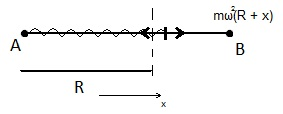
\includegraphics[height=30mm]{3_33.jpg}\\
	$\vec k = k \vec n, \quad \vec n = \vec e_x \cos \alpha + \vec e_y \cos \beta + \vec e_x \cos \gamma $\\
	$k = \frac{\omega}{\upsilon}, \quad \cos \alpha = \frac{\upsilon}{\upsilon_1} \quad \cos \beta = \frac{\upsilon}{\upsilon_2} \quad \cos \gamma = \frac{\upsilon}{\upsilon_3} $\\
	$\vec k = \omega\left( \frac{\vec e_x}{\upsilon_1} + \frac{\vec e_y}{\upsilon_2} + \frac{\vec e_z}{\upsilon_3} \right)$\\
}

